\chapter{Implementation}
% Explain the implementation specifics and elaborate on some architectural decisions made in 4

For our implementation it was important that we do not reinvent the wheel at each corner.

Choosing a DLT platform was not easy, as there were many options for Blockchains/DLTs but very few that were more or
less directly applicable to our thesis, which is IoTeX but its permissionless nature is not of good to us, as we would
like our network to be permissioned, which is another increase in security.

Another aspect of was the quality of documentation. In order not to waste time trying to figure out the source code,
documentation of it is important.

The choice of physical devices, whose purpose lies with demonstrating our platforms capabilities, fell to the following.
For the controller nodes, we will be using Raspberry Pi 4B, demonstrating portability and the use of embedded Linux,
reflecting future capabilities. It is able to coordinate with the chosen blockchains.

For the edge nodes we have decided to use the Raspberry Pi Pico, which is a capable and demonstrative microcontroller
unit, MCU, able to run CircuitPython, as well as simple bare-metal software.

\section{Configuration and Management Database} % (fold)
\label{sec:Configuration and Management Database}

\begin{figure}
	\begin{center}
		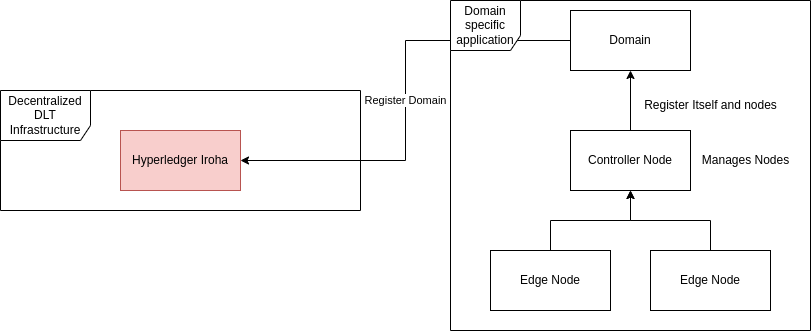
\includegraphics[width=0.95\textwidth]{figures/cmdb-iroha-architecture.png}
	\end{center}
	\caption{CMDB using Hyperledger Iroha}
	\label{fig:cmdb-iroha-architecture}
\end{figure}

In order to manage a fleet of devices, which consist of different layers, as mentioned in Section~\ref{sec:System Components},
we will rely on a Configuration / Management Database and for the sake of decentralization, it will entail using a DLT.

The (current) choice falls upon Hyperledger Iroha, more specifically version 2, which is a rewrite from the original.
As explained in Section~\ref{sec:Blockchains}, Iroha is permissioned and allows creation of domains, accounts, as well
as the minting and burning of assets.
We tried to avoid having a permissionless blockchain, as well a one, that relied on cryptocurrencies for transactions,
such as Ethereum, as we do not aim to discourage unnecessary writes to the blockchain, as every write will be fulfilled
by a recognized member of a registered domain.

Figure~\ref{fig:cmdb-iroha-architecture} gives a high-level overview over the CMDB architecture.

% section Configuration and Management Database (end)

\section{Device onboarding} % (fold)
\label{sec:Device onboarding}

For sake of simplicity, an AAA server and process will be assumed and therefore no secure onboarding will be included.

\begin{figure}
	\begin{center}
		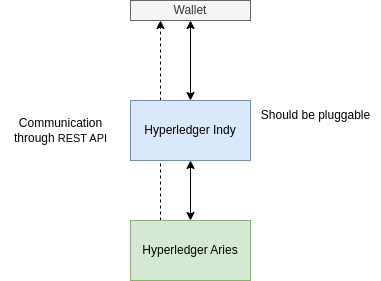
\includegraphics[width=0.95\textwidth]{figures/credential-architecture.png}
	\end{center}
	\caption{Credential Management Architecture}
	\label{fig:credential-architecture}
\end{figure}

% section Device onboarding (end)
